\documentclass{article}
\usepackage[utf8]{inputenc}
\usepackage{geometry}
\usepackage{graphicx}
\usepackage{pgfplots}
\usepackage{amsmath}
\usepackage{amssymb}
\usepackage{amsfonts}
\usepackage{mdframed}
\usepackage{amsthm}
\usepackage{physics}
\usepackage{derivative}
\usepackage{hyperref}
\usepackage{wrapfig}
\renewcommand{\theenumi}{\roman{enumi}}

\geometry{a4paper, left=2cm, right=2cm, top=1cm, bottom=2cm}

\pgfplotsset{compat=1.18}
\begin{document}

\begin{minipage}{0.7\textwidth}
    \small \textbf{ASTROFÍSICA GENERAL}  \\
    \small {Facultad de Ciencias, Universidad Nacional Autónoma de México} \\
    \small {Profesor: Margarita Rosado Solis} \\
    \small {Ayudante: Isidro Ramírez Ballinas}\\
    \small {Fecha de entrega: 10 de Octubre de 2024} \\
    \small {Nombre completo: Andrés López González} \\
    \small {Tarea número V}
\end{minipage}
\hfill
\begin{minipage}{0.12\textwidth}
    
\includegraphics[width=\linewidth]{logo_universidad}
\end{minipage}

\section*{Preguntas Semana V}

\subsection{Formación de la línea de 21 cm del hidrógeno neutro}
La línea de 21 cm es una emisión de radio producida por el hidrógeno neutro ($H I$) cuando hay un cambio en el estado de los espines del protón y el electrón en el átomo. En su estado más bajo de energía, los espines del electrón y el protón pueden estar alineados (espín paralelo, estado de mayor energía) o antialineados (espín antiparalelo, estado de menor energía). Cuando los espines pasan del estado alineado al antialineado, el átomo emite una fotón con una longitud de onda de 21 cm, correspondiente a una frecuencia de 1420 MHz.
\begin{figure}[h]
    \centering
    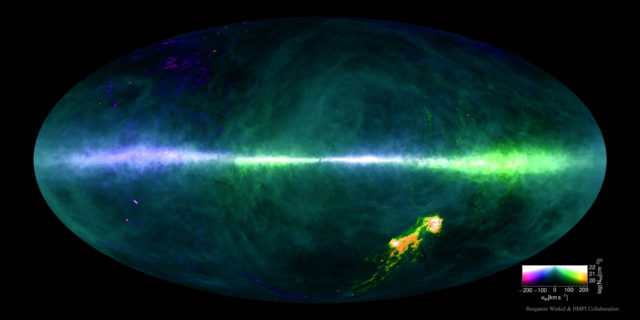
\includegraphics[width=0.5\linewidth]{21cm.png}
    \caption{La emisión del hidrógeno neutro a 21 cm.}
    \label{fig:enter-label}
\end{figure}
Aunque la regla de selección prohíbe transiciones en las que el cambio de espín sea no nulo ($\Delta S \neq 0$), esta transición ocurre debido a un efecto conocido como transición hiperfina, que se debe a la interacción magnética entre el espín del protón y del electrón. En condiciones normales, este tipo de transición es extremadamente rara y solo ocurre aproximadamente cada 10 millones de años para un átomo de hidrógeno aislado. Sin embargo, en el espacio interestelar, donde el hidrógeno es abundante y los tiempos son lo suficientemente largos, esta emisión se puede detectar.

Condiciones de temperatura y presión: En regiones con baja densidad y temperatura, como en el medio interestelar, las colisiones entre átomos de hidrógeno son muy escasas, lo que permite que estas transiciones ocurran y se detecten. En condiciones de alta presión y temperatura, las colisiones frecuentes entre átomos de hidrógeno pueden provocar transiciones inducidas entre los estados de espín, lo que aumenta la tasa de emisión y violación de la regla de selección.

\subsection{Presión de degeneración de neutrones y electrones}
La presión de degeneración es un efecto cuántico que aparece en sistemas extremadamente densos, como estrellas enanas blancas y estrellas de neutrones. Esta presión evita el colapso gravitacional de estos cuerpos, debido al principio de exclusión de Pauli, que prohíbe que dos fermiones ocupen el mismo estado cuántico.

Presión de degeneración de electrones: Se da en las enanas blancas, donde la densidad es lo suficientemente alta para que los electrones se degeneren (todos los niveles cuánticos hasta un cierto límite están ocupados). Esta presión es independiente de la temperatura y es la responsable de sostener a las enanas blancas contra la gravedad.

Presión de degeneración de neutrones: En una estrella de neutrones, la densidad es aún mayor, y los neutrones se degeneran. En este caso, la presión de degeneración de neutrones es mucho mayor que la de los electrones porque los neutrones tienen más masa. Esta presión soporta el colapso gravitacional de estrellas más masivas que las que forman enanas blancas.

Diferencia principal: La presión de degeneración de los neutrones es más fuerte debido a su mayor masa en comparación con los electrones, lo que hace que las estrellas de neutrones sean mucho más compactas que las enanas blancas. La presión de degeneración de neutrones es capaz de soportar objetos mucho más masivos.

\subsection{Cúmulo Pismis 24}
El cúmulo Pismis 24 es un cúmulo abierto ubicado en la nebulosa NGC 6357, conocida como la "Nebulosa de la Guerra y la Paz", en la constelación de Escorpión. Este cúmulo contiene algunas de las estrellas más masivas conocidas, como Pismis 24-1, que originalmente se pensaba que tenía una masa superior a 200 veces la masa del Sol, pero estudios posteriores mostraron que es un sistema estelar múltiple, compuesto por al menos tres estrellas masivas.

Las estrellas más masivas en Pismis 24 tienen masas entre 60 y 100 veces la masa del Sol. Las observaciones de estas estrellas se realizaron a través de telescopios ópticos y espectroscopía. La evidencia de sus masas proviene del análisis de sus espectros estelares, que permite determinar la temperatura y luminosidad de las estrellas. A partir de estos datos, se pueden usar modelos de evolución estelar para estimar sus masas.

Evidencias y técnicas:
\begin{enumerate}
\item Se utilizan observaciones espectroscópicas y fotométricas.
\item Comparando las líneas espectrales con modelos teóricos de evolución estelar.
\item Las estrellas masivas emiten intensamente en el espectro ultravioleta, lo que ayuda a identificar su tipo espectral y estimar su masa.
\end{enumerate}

\textbf{Curiosidad adicional.}\\
El Auditorio Paris Pismis es un espacio de la Universidad Nacional Autónoma de México (UNAM), nombrado en
\begin{wrapfigure}{l}{0.25\textwidth}
    \centering
    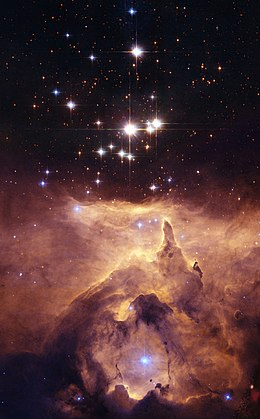
\includegraphics[width=0.5\linewidth]{pismis.png}
    \caption{Nebulosa Pismis 24 de la nebulosa NGC 6357}
\end{wrapfigure}
honor a Paris Pismis, una destacada astrónoma de origen turco-armenio que trabajó en México y contribuyó significativamente a la astronomía. Paris Pismis fue la primera mujer en obtener un doctorado en matemáticas y ciencias en Turquía y luego se trasladó a México, donde trabajó en el Instituto de Astronomía de la UNAM.

Su labor se destacó en la observación y estudio de cúmulos estelares y galaxias, y el cúmulo Pismis 24 lleva su nombre debido a su descubrimiento. El cúmulo está ubicado en la nebulosa NGC 6357, y como mencioné anteriormente, contiene estrellas masivas.
El auditorio en la UNAM lleva su nombre en reconocimiento a su legado en la astronomía, particularmente en la investigación de objetos estelares. Aunque no tiene una relación directa con el cúmulo Pismis 24, ambos están vinculados a la misma persona, lo que resalta la influencia de Paris Pismis en el campo de la astronomía.

\end{document}
